\section{Аналіз предметної області та опис сайту}
\subsection{Аналіз предметної області}
\subsubsection{Глосарій проекту}
\begin{enumerate}
    \item Замовник --- фізична чи юридична особа, розпорядник грошових коштів, який замовляє певні товари, або подає заявку про придбання чи замовлення товарів у майбутньому. 
    \item Адміністратор --- фізична особа, яка здійснює роботу з якісного і ефективного обслуговування відвідувачів. 
    \item Користувач --- відвідувач сайту, замовник та/або адміністратор. 
    \item Замовлення --- запит, який створюється замовником адміністратору й зазначає тип, кількість, якість, ціну та іншу інформацію про товари, які перший має намір придбати у останнього. 
    \item Товар --- це продукт праці, виготовлений з метою обміну або продажу.
    \item Звіт --- цифровий документ з інформацією про виконання певних замовлень. 
\end{enumerate}

\subsection{Опис сайту}
\subsubsection{Призначення сайту}
Інтернет-магазин <<\thesitename>> це потужний канал збуту, який розширює спектр послуг для клієнтів.
Це ефективний інструмент залучення нових клієнтів і партнерів c різних міст і регіонів через Інтернет.

Основне призначення даного інтернет-магазину --- демонстрація і продаж продукції.
Проект дозволяє:
\begin{itemize}
    \item легко оновлювати інформацію та супровідні графічні матеріали, гнучко реагувати на зміну попиту і визначати цінову політику;
    \item можливість дізнатися більше про своїх покупців (при здійсненні покупки клієнт обов'язково заповнює реєстраційну форму, в яку за бажанням можна включити і ряд питань, що стосуються маркетингової сфери);
    \item формувати базу клієнтів, які вже скористалися послугами електронного магазину.
\end{itemize}

Ряд істотних особливостей інтернет-магазину дозволяє використовувати його ефективніше, ніж традиційні рекламні технології:
\begin{itemize}
    \item доступність отримання інформації про продукцію компанії з будь-якої точки світу для будь-якого користувача мережі Інтернет;
    \item невисока вартість реклами в Інтернет, а також можливість направити рекламну кампанію на цільову аудиторію;
    \item точна інформація про популярність тих чи інших товарів;
    \item можливість оперативного внесення змін і доповнень в інформаційні матеріали на сервері і легкої зміни рекламних елементів без фінансових втрат;
    \item безперервна ефективна робота інтернет-магазину.
\end{itemize}

\subsubsection{Функціонал сайту}
Функціонал сайту відповідає функціональним вимогам, представленим у розділі~\ref{section:requirements_functional}.

\subsubsection{Особливості сайту}
Особливістю сайту є легкий дизайн у стилі <<material>> --- інтерфейс, поведінка і вигляд якого наслідують правила поведінки і вигляду паперових карток в реальному житті~(рисунок~\ref{fig:site_main}). 

В даному інтернет-магазині товари представлені картками з назвою товару, його графічним зображенням, описом та ціною.

\begin{figure}[H]
    \centering
    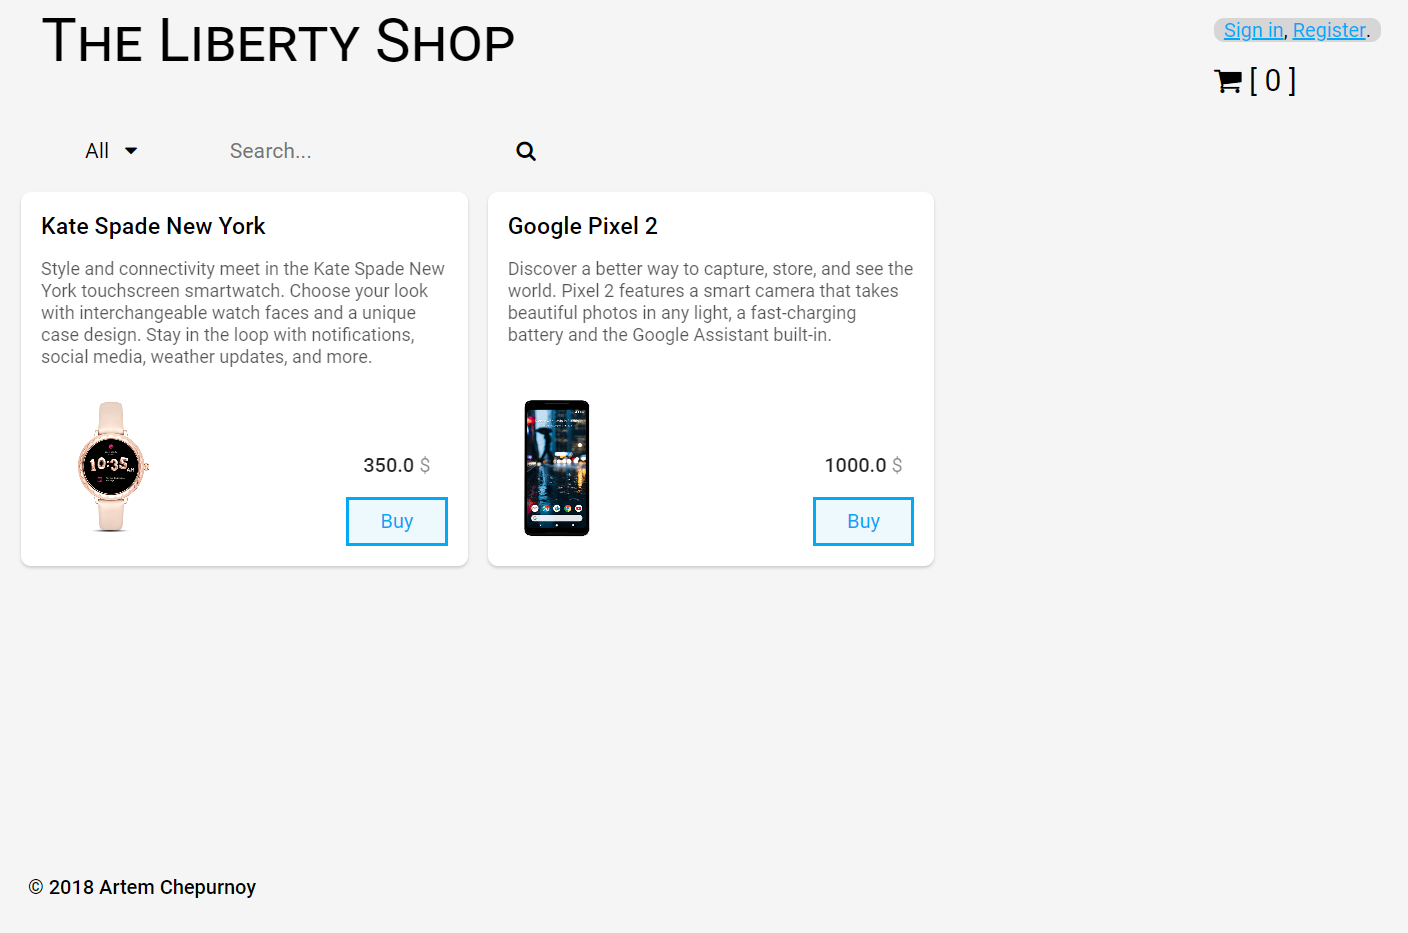
\includegraphics[width=0.8\textwidth]{screen_product__list}
    \caption{Головна сторінка ресурсу}
    \label{fig:site_main}
\end{figure}

Сайт має дуже просту та зрозумілу структуру:
\begin{itemize}
    \item головна сторінка, яка складається з елементів: пошук, вибір категорії продукту.
    \item карта клієнта;
    \item форма реєстрації.
\end{itemize}

Сайт написаний на чистому HTML5 та CSS з серверною частиною на PHP та SQLite, що дозволяє забезпечити високу швидкість завантаження сайту і низьке споживання ресурсів. 
